\pdfoutput=1
\PassOptionsToPackage{pdftex,
pdfversion=1.7,
pdfencoding=auto,
pdfnewwindow=true,
pdfusetitle=true,
%psdextra=true,
%pdftoolbar=true,
%pdfmenubar=true,
bookmarks=true,
bookmarksnumbered=true,
bookmarksopen=true,
pdfpagemode=UseThumbs,
bookmarksopenlevel=1,
pdfpagelabels=false,
breaklinks=true
}{hyperref}
\PassOptionsToPackage{usenames,dvipsnames,table}{xcolor}
\documentclass[aps,english,superscriptaddress,onecolumn,twoside,longbibliography,pra,floatfix,fleqn,nofootinbib]{revtex4-1}%

% packages
\usepackage[OT1]{fontenc}
\usepackage{amsfonts}
\usepackage{amssymb}
\usepackage{amsthm}
\usepackage[intlimits,fleqn]{amsmath}
\usepackage{bm}
\usepackage{graphicx}
%\usepackage{adjustbox}
\usepackage[normalem]{ulem} %for sout
\usepackage{paralist}
\usepackage{microtype}
\usepackage{float}% (not with floatrow)
\usepackage{wrapfig}
\usepackage{array}
\usepackage{ragged2e}%for justifying text in tables
\usepackage{tabularx}
\usepackage{booktabs}
\usepackage{comment}
%\usepackage{showkeys}
\usepackage[intlimits,fleqn]{mathtools} %for mathclap and prescript and more. Learning to love this package. And DeclarePairDelimeter!

% tables stuff
\newcolumntype{R}{>{\raggedleft\arraybackslash}X}
\newcolumntype{C}{>{\centering\arraybackslash}X}
\newcolumntype{L}{>{\raggedright\arraybackslash}X}
\newcolumntype{J}{>{\justifying\arraybackslash}X}
\usepackage{adjustbox}
\usepackage{multirow}
\newcolumntype{T}[2]{%
    >{\adjustbox{angle=#1,lap=\width-(#2)}\bgroup}%
    l%
    <{\egroup}%
}
\setcounter{MaxMatrixCols}{30}

\usepackage{verbatim} %for comment command

% colours and hyperlink stuff
\usepackage[usenames,dvipsnames,table]{xcolor}
\definecolor{purple}{RGB}{128,0,128}
\definecolor{ultramarine}{RGB}{63, 0, 255}
\definecolor{medblue}{RGB}{0, 0, 100}
\definecolor{panblue}{RGB}{0,24,150}
\definecolor{carmine}{RGB}{150, 0, 24}
\definecolor{gray}{RGB}{150, 150, 150}
\usepackage[pdftex,pdfversion=1.7,pdfencoding=auto,pdfnewwindow=true,pdfusetitle=true,bookmarks=true,bookmarksnumbered=true,bookmarksopen=true,pdfpagemode=UseThumbs,bookmarksopenlevel=1,pdfpagelabels=false,breaklinks=true]{hyperref}
\hypersetup{colorlinks,
linkcolor=carmine,
citecolor=medblue,
urlcolor=panblue,
anchorcolor=OliveGreen}



% coloured text
\newcommand*{\mred}[1]{{\color{RawSienna}{\mathbf{#1}}}}
\newcommand*{\mgreen}[1]{{\color{OliveGreen}{\mathbf{#1}}}}
\newcommand*{\tred}[1]{{\color{carmine}{\textbf{#1}}}}
\newcommand*{\tblue}[1]{{\color{MidnightBlue}{\textbf{#1}}}}
\newcommand*{\tpurp}[1]{{\color{Plum}{{#1}}}}

% cleveref stuff
\usepackage[capitalise]{cleveref}
\Crefname{eqs}{Eqs.}{Eqs.}
\creflabelformat{eqs}{(#2#1#3)}
\crefrangelabelformat{equation}{(#3#1#4-#5#2#6)}
\Crefmultiformat{equation}{Eqs.~(#2#1#3}{,#2#1#3)}{,#2#1#3}{,#2#1#3)}
\crefrangelabelformat{eqs}{(#3#1#4-#5#2#6)}
\Crefmultiformat{eqs}{Eqs.~(#2#1#3}{,#2#1#3)}{,#2#1#3}{,#2#1#3)}
\Crefname{example}{Example}{Examples}
\Crefname{section}{Sec.}{Secs.}



% theorem environments
\newtheorem{theorem}{Theorem}
\newtheorem{lemma}[theorem]{Lemma}
\newtheorem{claim}[theorem]{Claim}
\newtheorem{conjecture}[theorem]{Conjecture}
\newtheorem{corollary}[theorem]{Corollary}
\newtheorem{definition}[theorem]{Definition}
\theoremstyle{definition}
%\newtheorem{example}{Example}
\newtheorem{exercise}{Exercise}
\newtheorem{notation}[theorem]{Notation}
\newtheorem{problem}[theorem]{Problem}
\newtheorem{remark}[theorem]{Remark}

\newcounter{example}[section]
\newenvironment{example}[1][]{\refstepcounter{example}\par\medskip
   \noindent \textbf{Example~\theexample}\hspace{1em}\rmfamily#1}{\par\medskip\par}
\Crefname{example}{Example}{Examples}
\creflabelformat{example}{#2#1#3}
\crefrangelabelformat{example}{#3#1#4-#5#2#6}
\Crefmultiformat{example}{Examples~#2#1#3}{, #2#1#3}{, #2#1#3 }{and #2#1#3}
\renewcommand{\theexample}{\arabic{example}}

% macros for our notation
\newcommand{\p}[2][]{{P_{#1}}\parenths{#2}}
\newcommand{\pfunc}[1]{P_{#1}}
\newcommand{\An}[2][]{{\mathsf{An}_{#1}}\parenths{#2}}
\newcommand{\Pa}[2][]{{\mathsf{Pa}_{#1}}\parenths{#2}}
\newcommand{\Ch}[2][]{{\mathsf{Ch}_{#1}}\parenths{#2}}
\newcommand{\SmallNamedFunction}[3][]{\operatorname{\mathsf{#2}}_{#1}\parenths{#3}}
\newcommand{\subgraph}[2][]{\SmallNamedFunction[#1]{SubDAG}{#2}}
\newcommand{\ansubgraph}[2][]{\SmallNamedFunction[#1]{AnSubDAG}{#2}}
\newcommand{\nodes}[1]{\SmallNamedFunction{Nodes}{#1}}
\newcommand{\obsnodes}[1]{\SmallNamedFunction{ObservedNodes}{#1}}
\newcommand{\latnodes}[1]{\SmallNamedFunction{LatentNodes}{#1}}
\newcommand{\inflations}[1]{\SmallNamedFunction{Inflations}{#1}}
\newcommand{\DAG}[1]{\SmallNamedFunction{DAG}{#1}}
\newcommand{\edges}[1]{\SmallNamedFunction{Edges}{#1}}
\newcommand{\aindep}{\perp} % for d-separation
\newcommand{\indep}{\perp\!\!\!\!\perp} % (conditional) independence
\newcommand{\cramp}[1]{\ensuremath{\mathord{#1}}}
\newcommand{\eql}{\cramp{=}}
\DeclarePairedDelimiter{\parens}{\lparen}{\rparen}
\DeclarePairedDelimiter{\parenths}{\lparen}{\rparen}
\DeclarePairedDelimiter{\braces}{\lbrace}{\rbrace}
\DeclarePairedDelimiter{\bracks}{\lbrack}{\rbrack}
\DeclarePairedDelimiter{\expec}{\langle}{\rangle}
\newcommand{\brackets}[1]{\braces*{#1}}

% more vertical spacing in multiline equations
\setlength{\jot}{6pt}





\begin{document}

\title{Expressible sets and expressible assignments}

\author{RWS}

%\date{}                                           % Activate to display a given date or no date

\maketitle
%\section{}
%\subsection{}

\section{Expressible sets}

\begin{example}[\tred{Incompatibility of Pienaar distribution with DAG \#16}]
\label{example:Pienaar}

Consider the DAG of \cref{fig:GDAG16}.  Henson, Lal and Pusey showed that this DAG is a candidate for being `interesting', that is, the compatible distributions satisfy constraints over and above the conditional independence relations that follow from d-separation relations in the DAG. 

% i.e. for which the set of distributions that are compatible with it is a strict subset of those with conditional independence relations that are implied by the d-separation criterion. 

% Pienaar subsequently showed that this was the case by demostrating that the following distribution is incompatible with the DAG:

\begin{figure}[htb]
\centering
\begin{minipage}[t]{0.4\linewidth}
\centering
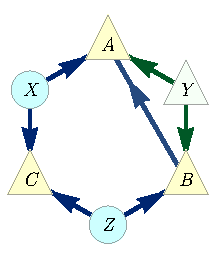
\includegraphics[scale=1]{scen16DAG.pdf}
\caption{DAG \#16 in Ref.~\cite{pusey2014gdag}.}\label{fig:GDAG16}
\end{minipage}
\hfill
\begin{minipage}[t]{0.5\linewidth}
\centering
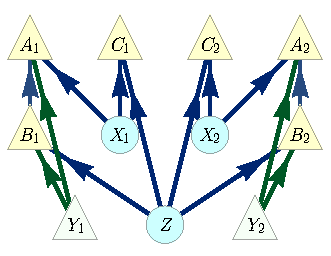
\includegraphics[scale=1]{scen16InflationDAG.pdf}
\caption{The Rocket inflation of \cref{fig:GDAG15}.}\label{fig:Inflated15}
\end{minipage}
\end{figure}

\citet{pianaar2016interesting} identified a distribution which satisfies the CI relations among the observed variables in DAG \#16, namely, $Y\indep C$ and $A\indep B | Y$~\cite{pusey2014gdag}, but is nonetheless incompatible with it:
\begin{align}\label{eq:pienaardistro}
    P^{\text{Pien}}_{A B C Y}:=\frac{[0000]+[0110]+[0001]+[1011]}{4},\quad\text{i.e.,}\quad P^{\text{Pien}}_{Y\! A B C}(y a b c):=\begin{cases}\tfrac{1}{4}&\text{if }  y\cdot c = a \text{ and }  (y \oplus 1)\cdot c = b, \\ 0&\text{otherwise}.\end{cases}
\end{align}
Note that we can rewrite Eq.~\eqref{eq:pienaardistro} as
\begin{align}
P^{\text{Pien}}_{A B C Y}= \frac{1}{2}([00]_{BC}+[11]_{BC})[0]_A [0]_Y + \frac{1}{2}([00]_{AC}+[11]_{AC}) [0]_B [1]_Y,
\end{align}
which makes it evident that the distribution can be described as follows: if $Y=0$, then $B$ and $C$ are in a maximally correlated state and $A=0$, while if $Y=1$, then $A$ and $C$ are maximally correlated and $B=0$.

Here, we will establish this incompatibility using the inflation technique.  To do so, we use the inflation of DAG \#16 depicted in \cref{fig:Inflated15}.  
%The expressible sets include $\{ A_1 B_1 C_2 Y_1 Y_2\}, \{A_2 B_2 C_1 Y_1 Y_2\}, \{A_2 B_2 C_2 Y_1 Y_2\}$ and $\{A_1 B_1 C_1 Y_1 Y_2\}$. 
To do so, we will make use of the fact that $\{ B_2 C_2 Y_2\}, \{ A_1 C_1 Y_1\}$ and $\{B_2 C_1 Y_2 \}$ are injectable sets, together with the fact that $\{ A_1 C_2 Y_1\}$ is an expressible set. 

We begin by demonstrating how the $d$-separation relations in the inflation imply that $\{ A_1 C_2 Y_1\}$ is expressible.  The expressibility of $\{ A_1 C_2 Y_1\}$ follows from the expressibility of $\{ A_1 B_1 C_2 Y_1\}$ and the fact that the distribution on the former can be obtained from the distribution on the latter by marginalization.  $\{ A_1 B_1 C_2 Y_1\}$ is expressible because the d-separation relation $A_1 \perp C_2 | B_1 Y_1$ implies that
\begin{align}
P_{A_1 B_1 C_2 Y_1} = \frac{P_{A_1 B_1 Y_1} P_{C_2 B_1 Y_1} }{P_{B_1 Y_1}},
\end{align}
and each of the sets $\{A_1 B_1 Y_1\}, \{C_2 B_1 Y_1\},$ and $\{B_1 Y_1\}$ are injectable.  
We therefore have 
\begin{align}
%P_{A_1 C_2 Y_1}(a_1 c_2 y_1) = \sum_{b_1} \frac{P_{A_1 B_1 Y_1}(a_1 b_1 y_1) P_{C_2 B_1 Y_1}(c_2 b_1 y_1) }{P_{B_1 Y_1}(b_1 y_1)},
P_{A_1 C_2 Y_1}(a c y) = \sum_{b} \frac{P^{\text{Pien}}_{A B Y}(a b y) P^{\text{Pien}}_{C B Y}(c b y) }{P^{\text{Pien}}_{B Y}(b y)},
\label{express1}
\end{align}

From the injectability of $\{ B_2 C_2 Y_2\}, \{ A_1 C_1 Y_1\}$ and $\{B_2 C_1 Y_2 \}$, we can infer that 
\begin{align}
%P_{B_2 C_2 |Y_2}(\cdot \cdot| 0)&= P^{\text{Pien}}_{BC|Y}(\cdot \cdot| 0) \nonumber\\
%P_{A_1 C_1  |Y_1}(\cdot \cdot| 1)&= P^{\text{Pien}}_{AC|Y}(\cdot \cdot| 1)\nonumber\\
%P_{B_2 C_1 |Y_2}(\cdot \cdot| 0)&= P^{\text{Pien}}_{BC|Y}(\cdot \cdot| 0) 
P_{B_2 C_2 |Y_2}(bc| y)&= P^{\text{Pien}}_{BC|Y}(bc|y) \nonumber\\
P_{A_1 C_1  |Y_1}(ac|y)&= P^{\text{Pien}}_{AC|Y}(ac|y)\nonumber\\
P_{B_2 C_1 |Y_2}(bc|y)&= P^{\text{Pien}}_{BC|Y}(bc|y) 
\end{align} 
which implies that
\begin{align}
P_{B_2 C_2 |Y_2}(\cdot \cdot| 0)&= \frac{1}{2}([00]_{B_2 C_2}+[11]_{B_2 C_2})\label{inj1}\\
P_{A_1 C_1  |Y_1}(\cdot \cdot| 1)&= \frac{1}{2}([00]_{A_1 C_1}+[11]_{A_1 C_1}) \label{inj2}\\
P_{B_2 C_1 |Y_2}(\cdot \cdot| 0)&= \frac{1}{2}([00]_{B_2 C_1}+[11]_{B_2 C_1})\label{inj3}
\end{align} 

For the expressible set $\{ A_1 C_2 Y_1\}$, Eq.~\eqref{express1} implies that
\begin{align}
%P_{A_1 C_2 Y_1}(a_1 c_2 y_1) = \sum_{b_1} \frac{P_{A_1 B_1 Y_1}(a_1 b_1 y_1) P_{C_2 B_1 Y_1}(c_2 b_1 y_1) }{P_{B_1 Y_1}(b_1 y_1)},
P_{A_1 C_2 |Y_1}(a c |y) &= \sum_{b} \frac{P^{\text{Pien}}_{A B Y}(a b y) P^{\text{Pien}}_{C B Y}(c b y) }{P^{\text{Pien}}_{B Y}(b y) P^{\text{Pien}}_{Y}(y)}\nonumber\\
&=\sum_{b} \frac{P^{\text{Pien}}_{A B |Y}(a b| y) P^{\text{Pien}}_{C B| Y}(c b |y) }{P^{\text{Pien}}_{B |Y}(b |y)},\label{A1C2Y1}
\end{align}
where we have simply used the definition of conditioning.  
%It follows that
%\begin{align}
%P_{A_1 C_2 |Y_1}(a c |1) =\sum_{b} \frac{P^{\text{Pien}}_{A B |Y}(a b| y) P^{\text{Pien}}_{C B| Y}(c b |y) }{P^{\text{Pien}}_{B |Y}(b |y)},
%\end{align}
%It will be useful in what follows to consider the joint probability for $A_1=0, C_2=0$ given $Y_1=1$
%\begin{align}
%P_{A_1 C_2 |Y_1}(00 |1) &=\sum_{b} \frac{P^{\text{Pien}}_{A B |Y}(0 b| 1) P^{\text{Pien}}_{C B| Y}(0 b |1) }{P^{\text{Pien}}_{B |Y}(b |1)}\nonumber\\
%&= \frac{P^{\text{Pien}}_{A B |Y}(0 0| 1) P^{\text{Pien}}_{C B| Y}(0 0 |1) }{P^{\text{Pien}}_{B |Y}(0 |1)}
%+  \frac{P^{\text{Pien}}_{A B |Y}(0 1| 1) P^{\text{Pien}}_{C B| Y}(0 1 |1) }{P^{\text{Pien}}_{B |Y}(1 |1)}\nonumber\\
%&= \frac{1}{4}\label{A1C2Y1}
%\end{align}

Now suppose that $Y_2=0$ and $Y_1=1$.  From Eq.~\eqref{inj3}, we infer that 
\begin{align}
\text{With probability 1/2,}\; B_2=0\; \text{and}\;C_1=0.
\end{align}
From Eq.~\eqref{inj1}, we infer that
\begin{align}
\text{if}\; B_2=0\; \text{then}\;C_2=0.
\end{align}
From Eq.~\eqref{inj2}, we infer that 
\begin{align}
\text{if}\; C_1=0\; \text{then}\;A_1=0.
\end{align}
These three results imply that 
\begin{align}
\text{The probability}\; p\; \text{that }\; C_2=0\; \text{and}\;A_1=0 \;\text{must be} \; \ge 1/2.
\end{align}
However, from Eq.~\eqref{A1C2Y1}, we infer that the probability of $C_2=0\; \text{and}\;A_1=0$ is only $p=1/4$.   
Explicitly, 
\begin{align}
P_{A_1 C_2 |Y_1}(00 |1) &=\sum_{b} \frac{P^{\text{Pien}}_{A B |Y}(0 b| 1) P^{\text{Pien}}_{C B| Y}(0 b |1) }{P^{\text{Pien}}_{B |Y}(b |1)}\nonumber\\
&= \frac{P^{\text{Pien}}_{A B |Y}(0 0| 1) P^{\text{Pien}}_{C B| Y}(0 0 |1) }{P^{\text{Pien}}_{B |Y}(0 |1)}
+  \frac{P^{\text{Pien}}_{A B |Y}(0 1| 1) P^{\text{Pien}}_{C B| Y}(0 1 |1) }{P^{\text{Pien}}_{B |Y}(1 |1)}\nonumber\\
&= \frac{1}{4}\label{A1C2Y1}
\end{align}
We have therefore arrived at a contradiction.  This establishes the incompatibility of the Pienaar distribution with DAG \#16.

\end{example}

\begin{comment}
 
We will here make use of the fact that $\{ A_1 B_1 C_2 Y_1 Y_2\}$ is an expressible set.  To demonstrate that this is the case, we make use of the d-separation relation $A_1 \perp C_2 \perp Y_2 | B_1 Y_1$ in the inflation to infer that
\begin{align}
P_{A_1 B_1 C_2 Y_1 Y_2} = \frac{P_{A_1 B_1 Y_1} P_{C_2 B_1 Y_1} P_{Y_2 B_1 Y_1}}{P_{B_1 Y_1}^2}.
\end{align}
We then use the d-separation relation $Y_2 \perp B_1 Y_1$ to decompose the final term of the numerator as
\begin{align}
P_{Y_2 B_1 Y_1} = P_{Y_2} P_{B_1 Y_1},
\end{align}
so that 
\begin{align}
P_{A_1 B_1 C_2 Y_1 Y_2} = \frac{P_{A_1 B_1 Y_1} P_{C_2 B_1 Y_1} P_{Y_2} }{P_{B_1 Y_1}}.
\end{align}
Because each of the sets $\{A_1 B_1 Y_1\}, \{C_2 B_1 Y_1\}, \{B_1 Y_1\}, \{ Y_2\}$ are injectable, it follows that the set $\{ A_1 B_1 C_2 Y_1 Y_2\}$ is expressible.  
Note that $\{ A_1 B_1 C_2 Y_1 Y_2\}$ is not preinjectable because we have used more than ancestral independences to prove its expressibility.
% Note that it is not preinjectable because $A_1$ has $X_1$ as ancestor, while $C_2$ has $X_2$ as ancestor [say more here].

We consider the case where $Y_2=0$ and $Y_1=1$.  

The injectable sets include $\brackets{A_1 B_1 C_1 Y_1}$ and $\brackets{A_2 B_1 C_2 Y_1}$.  They share the same  image on the original DAG, namely, the set of all observed variables, $\brackets{ABCY}$. It follows that
\begin{align}
P_{A_1 B_1 C_1 Y_1} = P_{A_2 B_1 C_2 Y_1} =P^{\text{Pien}}_{ABCY}.
\label{bridge1}
\end{align}

If $P^{\text{Pien}}_{ABCY}$ is compatible with the given inflation of DAG \#16, then by Lemma ?, $P_{A_1 B_1 C_1 Y_1}$ and $ P_{A_2 B_1 C_2 Y_1}$ are compatible with this inflation, and conversely if we can show incompatibility of the latter, we establish incompatibility of the former.  To show that $P^{\text{Pien}}_{ABCY}$ is indeed incompatible with the inflation of DAG \#16, we assume compatibility and derive a contradiction.

%With a slight rewriting of Eq.~\ref{eq:pienaardistro}, we have
Note first that we can rewrite Eq.~\eqref{eq:pienaardistro} as
\begin{align}
P^{\text{Pien}}_{A B C Y}= \frac{1}{2}([00]_{BC}+[11]_{BC})[0]_A [0]_Y + \frac{1}{2}([00]_{AC}+[11]_{AC}) [0]_B [1]_Y
\end{align}
It then follows from Eq.~\eqref{bridge1} that
\begin{align}
P_{A_1 C_1 | Y_1=1} = \frac{1}{2}([00]_{A_1 C_1}+[11]_{A_1 C_1}),\label{A1C1Y1e1}\\
P_{A_2 C_2 |Y_1=1} = \frac{1}{2}([00]_{A_2 C_2}+[11]_{A_2 C_2}).\label{A2C2Y1e1}
\end{align}
and that 
\begin{align}
P_{B_1 C_1 | Y_1=0} = \frac{1}{2}([00]_{B_1 C_1}+[11]_{B_1 C_1}),\label{B1C1Y1e0}\\
P_{B_1 C_2 |Y_1=0} = \frac{1}{2}([00]_{B_1 C_2}+[11]_{B_1 C_2}).\label{B1C2Y1e0}
\end{align}

Any distribution $P_{B_1 C_1 C_2 Y_1}$ which has marginals $P_{B_1 C_1 Y_1}$ and $P_{B_1 C_2 Y_1}$ that reproduce the conditional distributions of \cref{B1C1Y1e0} and \cref{B1C2Y1e0} respectively, must be such that 
\begin{align}
P_{B_1 C_1 C_2 | Y_1=0} = \frac{1}{2}([000]_{B_1 C_1 C_2}+[111]_{B_1 C_1 C_2})\label{B1C1C2Y1e0}.
\end{align}
The reason is that if $B_1$ and $C_1$ are perfectly correlated, as in \cref{B1C1Y1e0}, and $B_1$ and $C_2$ are perfectly correlated, as in \cref{B1C2Y1e0}, then $C_1$ and $C_2$ must be perfectly correlated as well.  \cref{B1C1C2Y1e0} ensures this: marginalizing this distribution over $B_1$, we obtain
\begin{align}
P_{C_1 C_2 | Y_1=0} = \frac{1}{2}([00]_{ C_1 C_2}+[11]_{C_1 C_2}).\label{C1C2Y1e0}
\end{align}

But the given inflation of DAG \#16 is such that $C_1 C_2$ and $Y_1$ are ancestrally independent, so that 
\begin{align}
P_{C_1 C_2 | Y_1} =P_{C_1 C_2},
\end{align}
and therefore $P_{C_1 C_2 | Y_1=0}=P_{C_1 C_2 | Y_1=1}$, so that we can infer from \cref{C1C2Y1e0} that
\begin{align}
P_{C_1 C_2 | Y_1=1} = \frac{1}{2}([00]_{ C_1 C_2}+[11]_{C_1 C_2})\label{C1C2Y1e1}.
\end{align}

Finally, we note that any distribution $P_{A_1 A_2 C_1 C_2 Y_1}$ which has marginals $P_{A_1 C_1 Y_1}$, $P_{A_2 C_2 Y_1}$, and $P_{C_1 C_2 Y_1}$ that reproduce the conditional distributions of \cref{A1C1Y1e1}, \cref{A2C2Y1e1} and \cref{C1C2Y1e1} respectively must be such that 
\begin{align}
P_{A_1 A_2 C_1 C_2 | Y_1=1} = \frac{1}{2}([0000]_{A_1 A_2 C_1 C_2}+[1111]_{A_1 A_2 C_1 C_2})\label{A1A2C1C2Y1e1}.
\end{align}
The reason is that if $A_1$ and $C_1$ are perfectly correlated, as in \cref{A1C1Y1e1}, and $A_2$ and $C_2$ are perfectly correlated, as in \cref{A2C2Y1e1}, and $C_1$ and $C_2$ are perfectly correlated, as in \cref{C1C2Y1e1}, then $A_1$ and $A_2$ must be perfectly correlated as well. 

Marginalizing \cref{A1A2C1C2Y1e1} over $C_1 C_2$, we obtain
\begin{align}
P_{A_1 A_2  | Y_1=1} = \frac{1}{2}([00]_{A_1 A_2}+[11]_{A_1 A_2})\label{A1A2Y1e1}.
\end{align}

Finally, we note that in the Parachute inflation of the Modified Triangle Scenario, $A_1$ is d-separated from $A_2$ given $Y_1$, which implies that $P_{A_1 A_2  | Y_1}=P_{A_1 | Y_1}P_{A_2  | Y_1}$.  This is inconsistent with \cref{A1A2Y1e1}, so we have derived a contradiction.

\color{black}
\end{comment}

\section{Instrumental inequality}

\subsection{Alternate form of the inequality}

Consider  the instrumental inequalities for binary variables:
\begin{align}
P_{XY|Z}(00|0) +  P_{XY|Z}(00|0) \le 1,\nonumber\\
P_{XY|Z}(10|0) +  P_{XY|Z}(11|1) \le 1,\nonumber\\
P_{XY|Z}(01|0) +  P_{XY|Z}(00|1) \le 1,\nonumber\\
P_{XY|Z}(11|0) +  P_{XY|Z}(10|1) \le 1. \label{II1}
\end{align}
It turns out that these can be obtained as special cases of the following set of causal compatibility inequalities for the instrumental scenario:
\begin{align}
P_{XY|Z} \le P_Y.
\label{II2}
\end{align}

To see that Eq.~\eqref{II2} implies \eqref{II1}, note that it implies 
\begin{align}
\forall x \forall z \forall y:  P_{XY|Z}(xy|z) \le P_Y(y),
\end{align}
which in turn implies that
\begin{align}
\forall x  \forall y:  P_{XY|Z}(xy|y) \le P_Y(y),
\end{align}
and 
\begin{align}
\forall x  \forall y:  P_{XY|Z}(xy|y\oplus 1) \le P_Y(y),
\end{align}
Summing over $y$ in each case, we obtain:
\begin{align}
\forall x : \sum_y  P_{XY|Z}(xy|y) \le 1,
\end{align}
and 
\begin{align}
\forall x : \sum_y  P_{XY|Z}(xy|y\oplus 1) \le 1,
\end{align}
respectively.  
These are the  instrumental inequalities for binary variables.  

%I have to think about whether the two conditions are in fact equivalent for binary variables.

The usual way of representing the instrumental inequality is as follows:
\begin{align}
\max_x \sum_y \max_z P(xy|z) \le 1.
\label{IIb1}
\end{align}
It too can be obtained as a special case of the following set of causal compatibility inequalities for the instrumental scenario:
\begin{align}
P_{YX|Z} \le P_Y.
\label{IIb2}
\end{align}

To see that Eq.~\eqref{IIb2} implies \eqref{IIb1}, note that it implies 
\begin{align}
\forall x \forall y \forall z: P_{YX|Z}(yx|z) \le P_Y (y),
\end{align}
which in turn implies 
\begin{align}
\forall x \forall y :\max_z P_{YX|Z}(yx|z) \le P_Y (y),
\end{align}
and therefore
\begin{align}
\forall x : \sum_y \max_z P_{YX|Z}(yx|z) \le 1,
\end{align}
which entails finally 
\begin{align}
\max_x \sum_y \max_z P_{YX|Z}(yx|z) \le 1,
\end{align}
which is the standard form of the instrumental inequality.

\subsection{Deriving the instrumental inequality using inflation technique and {\em expressible assignments}}



Consider the instrumental scenario, depicted in Fig.~\ref{fig:instrumental}, and the inflation thereof depicted in Fig. \ref{fig:InflatedInstrumental}.
\begin{figure}[htb]
\centering
\begin{minipage}[h!]{0.4\linewidth}
\centering
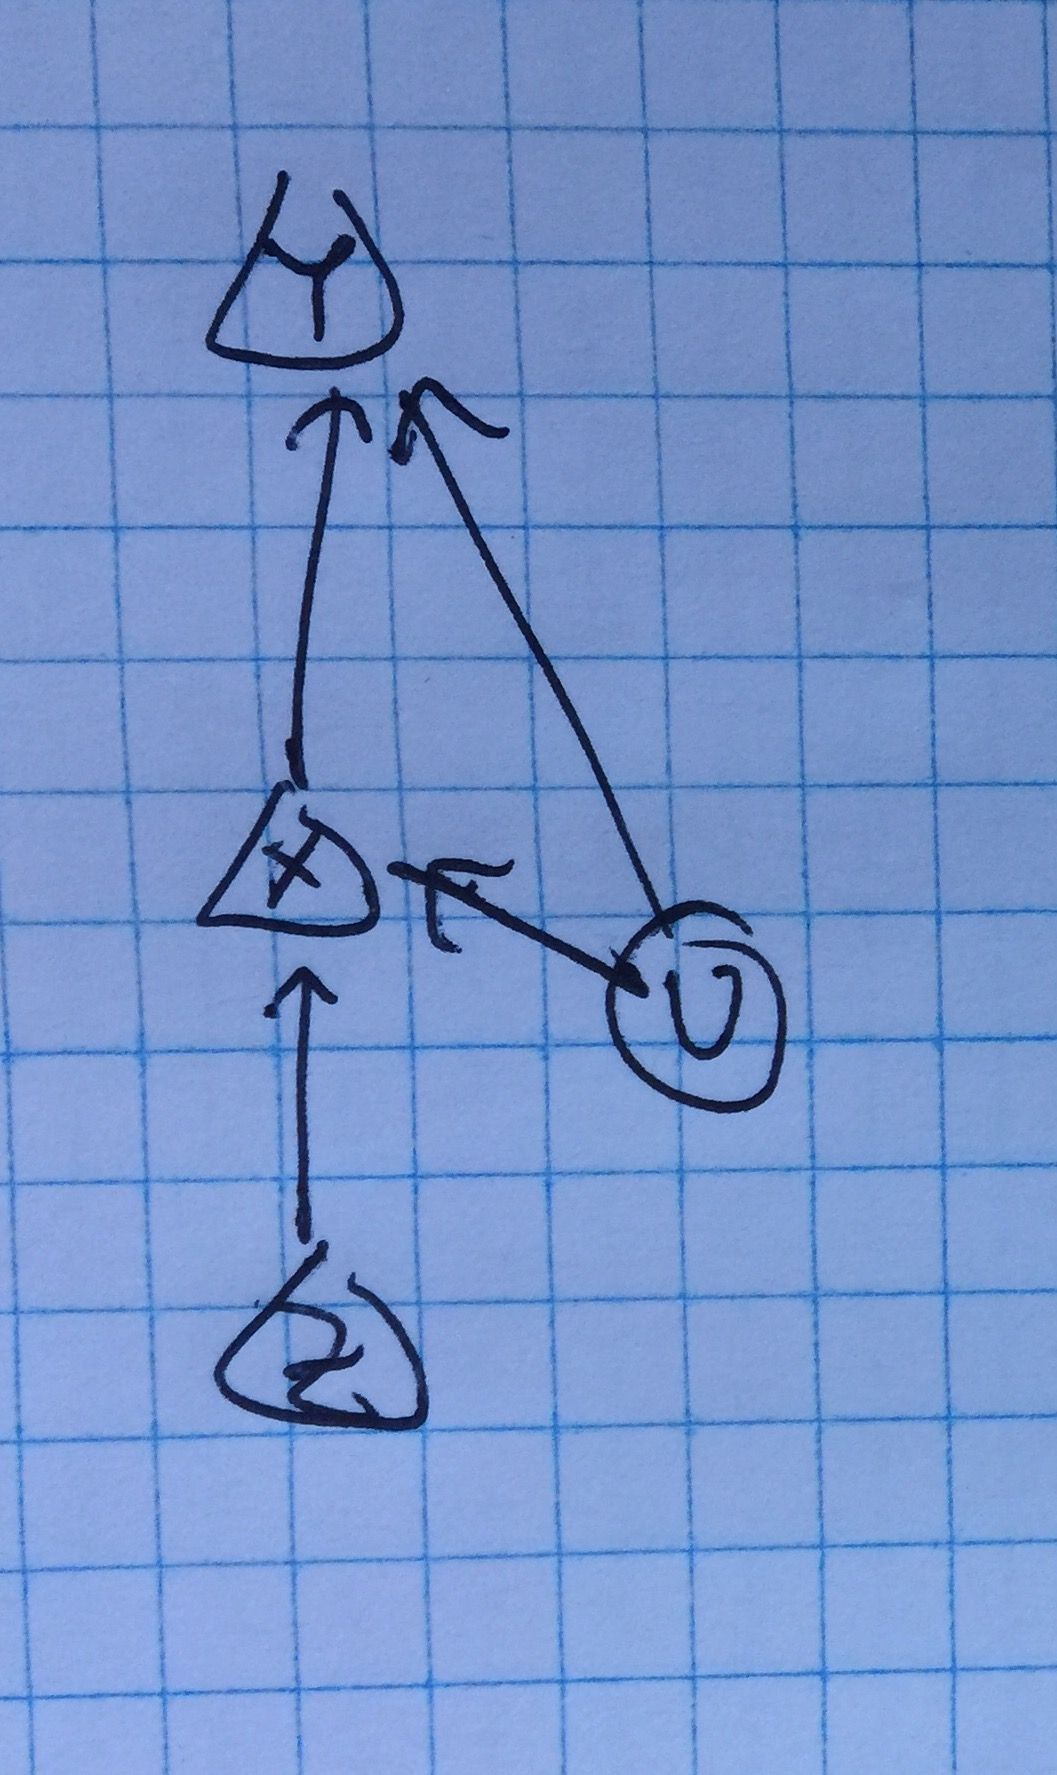
\includegraphics[scale=0.1]{Instrumental.jpg}
\caption{The instrumental scenario.}\label{fig:instrumental}
\end{minipage}
\hfill
\begin{minipage}[htb]{0.5\linewidth}
\centering
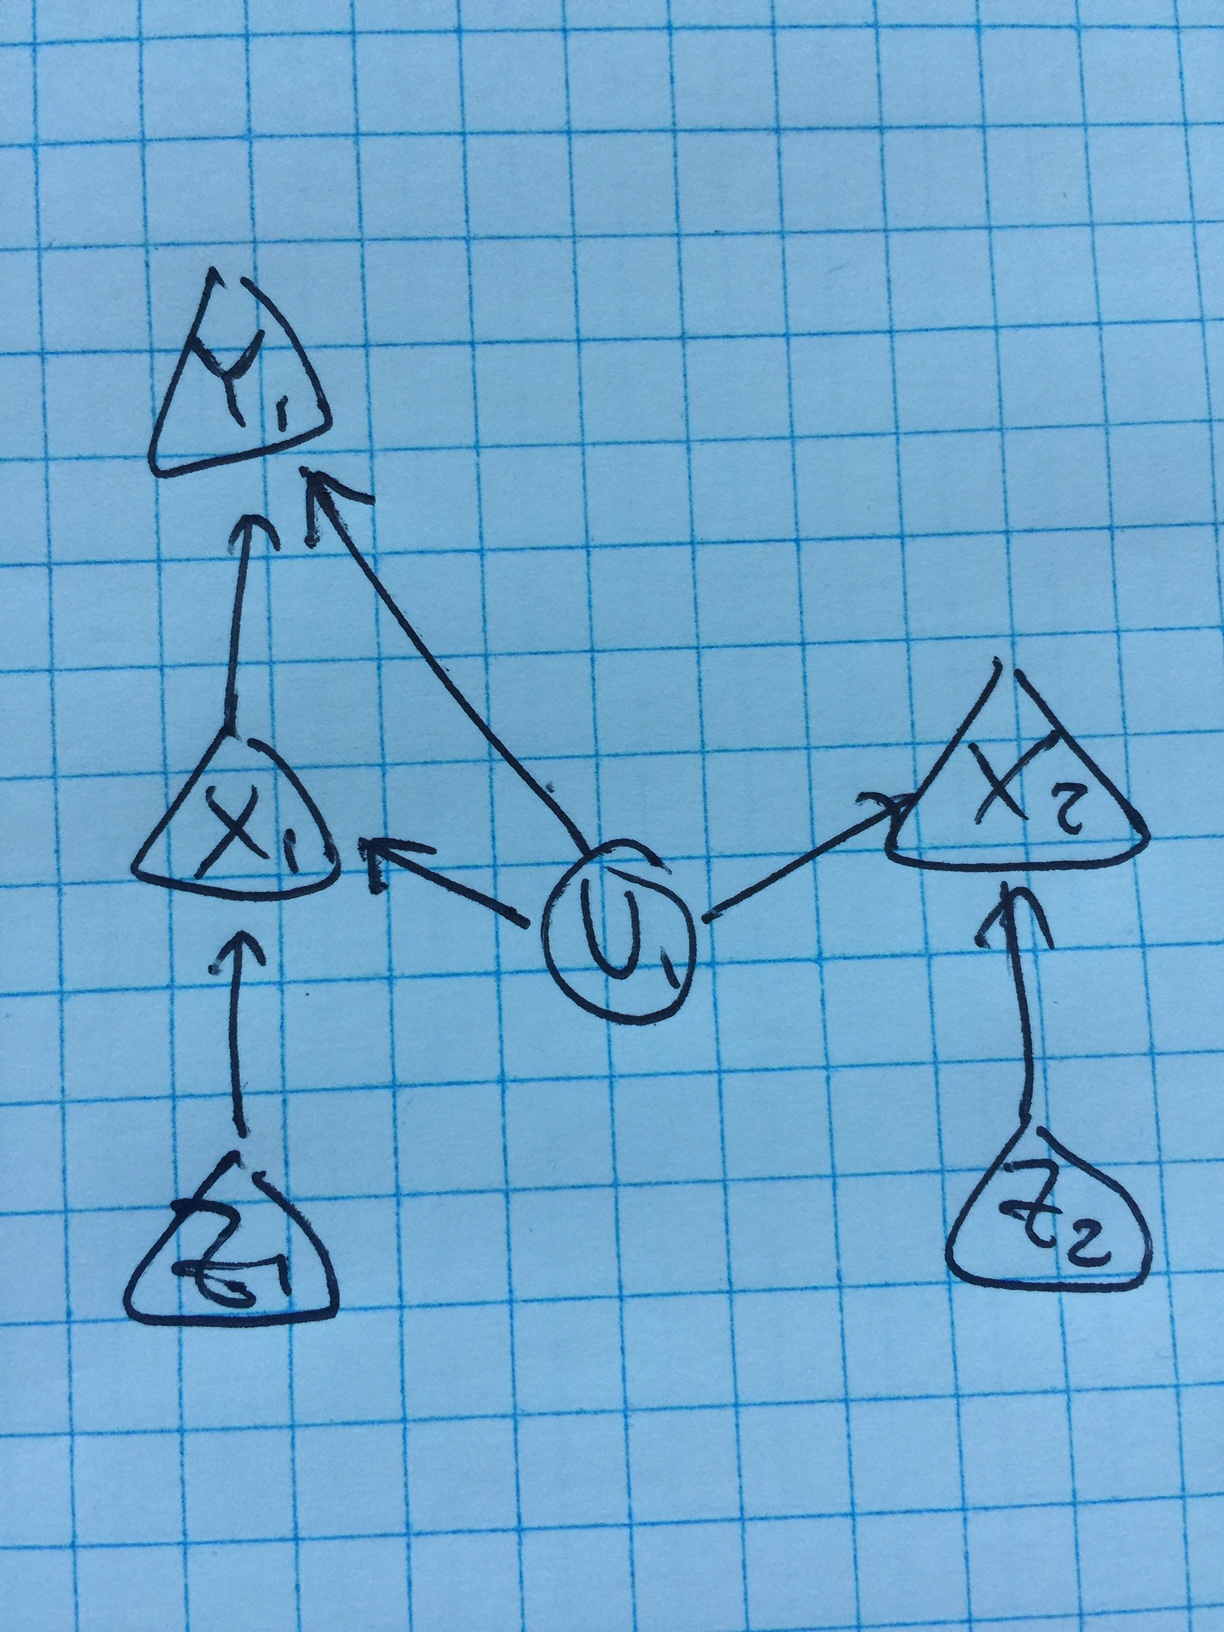
\includegraphics[scale=0.1]{InstrumentalInflation.jpg}
\caption{The Greyhound inflation of the instrumental scenario.}\label{fig:InflatedInstrumental}
\end{minipage}
\end{figure}

\begin{figure}[h!]
\centering
\begin{minipage}[t]{0.4\linewidth}
\centering
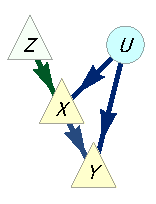
\includegraphics[scale=1]{InstrumentalDAGpearl.pdf}
\caption{The instrumental scenario.}\label{fig:instrumental}
\end{minipage}
\hfill
\begin{minipage}[htb]{0.5\linewidth}
\centering
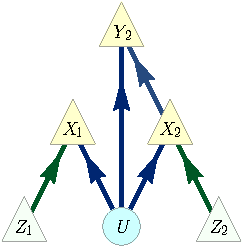
\includegraphics[scale=1]{instrumentalvariant.pdf}
\caption{The Greyhound inflation of the instrumental scenario, with the opposite labelling convention to the one I use below.}\label{fig:InflatedInstrumental}
\end{minipage}
\end{figure}

It is straightforward to verify that 
\begin{align}
P_{Y_1 Z_2 |X_2 X_1} ( \cdot \cdot | xx) = P_{Y Z |X} ( \cdot \cdot | x)
\label{exass1}
\end{align}

 In this case, we say that $P_{Y_1 Z_2 |X_2 X_1}$ is an {\em expressible assignment}.
 
 Note that Eq.~\eqref{exass1} implies that 
  \begin{align}
\frac{P_{Y_1 Z_2 X_2 X_1} ( \cdot \cdot xx)}{P_{X_1}(x)P_{X_2}(x)} = \frac{P_{Y Z X} ( \cdot \cdot x)}{P_{X}(x)},
\end{align}
and because $X_1$ and $X_2$ are injectable, we infer that 
 \begin{align}
P_{Y_1 Z_2 X_2 X_1} ( \cdot \cdot xx) = P_{Y Z X} ( \cdot \cdot x),
\end{align}
so $P_{Y_1 Z_2 X_2 X_1} ( \cdot \cdot xx)$ is also an expressible assignment. 

The d-separation relation $Y_1 \perp Z_2 | X_1 X_2$ in the inflation implies that 
\begin{align}
\sum_{X_1,X_2}P_{Y_1 Z_2 X_2 X_1}  = P_{Y_1} P_{Z_2}
%\sum_{x_1,x_2}P_{Y_1 Z_2 X_2 X_1} ( \cdot \cdot x_1 x_2)
\end{align}
This can be rewritten as
\begin{align}
\forall  y_1 \forall z_2 : \sum_{x}P_{Y_1 Z_2 X_2 X_1} ( y_1 z_2 x x) + \sum_{x_1 \ne x_2}P_{Y_1 Z_2 X_2 X_1} ( \cdot \cdot x_1 x_2)  \le P_{Y_1}(y_1) P_{Z_2}(z_2)
\end{align}
which implies that
\begin{align}
\forall  y_1 \forall z_2 : \sum_{x}P_{Y_1 Z_2 X_2 X_1} ( y_1 z_2 x x)   \le P_{Y_1}(y_1) P_{Z_2}(z_2).
\end{align}
Given that every term in the sum on the LHS is positive, the inequality holds for each such term,
\begin{align}
\forall  y_1 \forall z_2 : \forall x: P_{Y_1 Z_2 X_2 X_1} ( y_1 z_2 x x)   \le P_{Y_1}(y_1) P_{Z_2}(z_2).
\end{align}
Conditioning on $Z_2$, we obtain
\begin{align}
\forall  y_1 \forall z_2 \forall x: P_{Y_1 X_2 X_1|Z_2 } ( y_1  x x|z_2 )   \le P_{Y_1}(y_1).
\end{align}

Finally, given that the singleton set $\{Y_1\}$ is an injectable set and given that $P_{Y_1 X_2 X_1|Z_2 } ( y_1  x x|z_2 ) $ is an expressible assignment (described in Eq.~\eqref{exass1}),  we conclude that
\begin{align}
\forall  y \forall z  \forall x: P_{Y X | Z } ( y x|z )   \le P_{Y}(y),
\end{align}
which we showed previously to imply the instrumental inequality.

\end{document}  